\hskip-0.9cm\begin{minipage}[t]{0.9\textwidth}
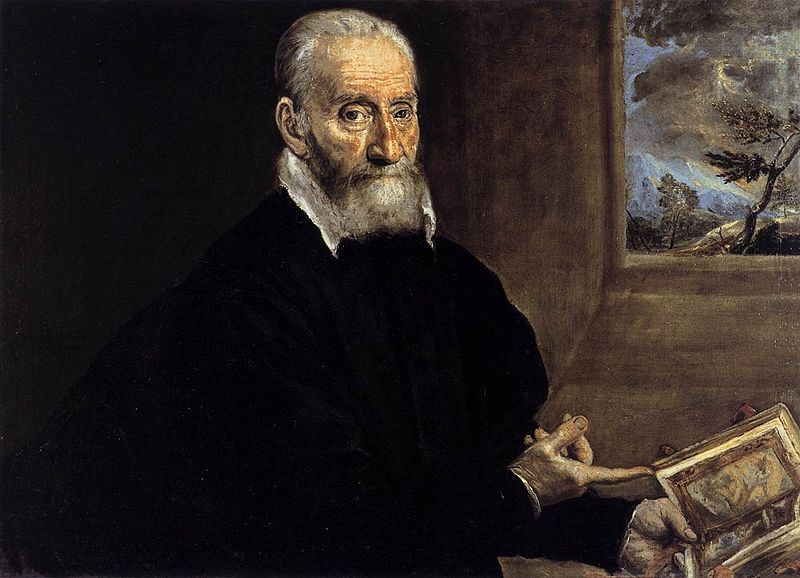
\includegraphics[width=1.15\textwidth]{julio}\\[-17pt]
\hfill\hfill{\tiny\bf FROM A PAINTING BY EL GRECO.}\\
\par
\end{minipage}
\setlength{\columnsep}{-10pt}
\setlength{\multicolsep}{0.9cm}
\vspace*{2\baselineskip}
\begin{center}\noindent
\large\bf GULIO CLOVIO
\end{center}
\begin{multicols}{3}
\leftskip0pt
\rightskip20pt
Giulio Clovio was born in Croatia. He was a native of Griane, a village near the town of Modru.[4] It is not known where he had his early training, but he may have studied art with monks at Fiume of Novi Bazar when he was young. [5]
He moved to Italy at age 18 and entered the household Cardinal Marino Grimani where he was trained as a painter. Between 1516 and ca 1523 Clovio may have lived with Marino in the residence of the latter’s uncle Cardinal Domenico Grimani in Rome. [6] Clovio studied under Giulio Romano during this early period. [7]

While a protege of Cardinal Domenico Grimani Clovio engraved medals and seals for him, as well as the Grimani Commentary Ms., an important early illuminated book (now Sir John Soane's Museum, London).
By 1524 Clovio was at Buda, at the Hungarian court of King Louis II, for whom he painted the ``Judgment of Paris'' and ``Lucretia''. After Louis' death in the Battle of Mohács, Clovio travelled to Rome where he continued his career.[8]

After 1527 he visited several monasteries of the Canons Regular of St. Augustine. In 1534 Clovio returned to the household of Cardinal Marino Grimani.[8] A year later Clovio may have followed Marino when the latter was appointed as a papal legate to Perugia, where Clovio is thought to have worked on illustrations for the Soane Manuscript written by Marino Grimani around that time. Clovio likely returned to Rome by the end of 1538 when he is known to have met with the writer Francisco de Hollanda.
\end{multicols}

\clearpage
